

\documentclass{article}
\usepackage[margin=1in]{geometry} 
\usepackage{amsmath,amsthm,amssymb,amsfonts, fancyhdr, color, comment, graphicx, environ}
\usepackage{xcolor}
\usepackage{mdframed}
\usepackage[shortlabels]{enumitem}
\usepackage{indentfirst}
\usepackage{hyperref}
\usepackage{graphicx}
\usepackage{caption}
\usepackage[serbian]{babel}
\renewcommand{\footrulewidth}{0.8pt}
\hypersetup{
    colorlinks=true,
    linkcolor=blue,
    filecolor=magenta,      
    urlcolor=blue,
}
\providecommand{\inlinecode}[1]{\texttt{#1}}


\pagestyle{fancy}



\newenvironment{problem}[2][Projekat]
    { \begin{mdframed}[backgroundcolor=gray!20] \textbf{#1 #2} \\}
    {  \end{mdframed}}


\newenvironment{solution}[2][]
    { \begin{mdframed}[backgroundcolor=gray!0] \textbf{#1 #2}}
    {  \end{mdframed}}

\newenvironment{eComment}[2][Zaključak]
    { \begin{mdframed}[backgroundcolor=gray!40] \textbf{#1 #2} \\}
    {  \end{mdframed}}



\lhead{Veljko Selaković}
\rhead{13S053NM} 
\chead{\textbf{Neuralne mreže - projekti}}
\rfoot{Elektrotehnički fakultet, Beograd}


\begin{document}
\title{\Large 13S053NM  \\[0.5cm]
        \bf\Large Neuralne mreže \\ -projekti-}
\author{\large Student: Veljko Selaković, 2019/0331\\
                \hspace{4.7cm} 0000/0000\ \\}

\makeatletter
    \begin{titlepage}
        \begin{center}
	   { 
\includegraphics[width=9cm]{etflogo.png}}
	   {\ \\ \ \\}
        \vbox{}\vspace{5cm}
            {\@title }\\[3cm] 
            {\@author}
            

        \end{center}
    \end{titlepage}
\makeatother%not necessary but looks fancy
    \begin{problem}{1}
    Klasifikovati date podatke primenom feedforward neuralne mreže. Prve dve kolone dataseta su zadati parametri dok treća označava pripadnost klasi. Dataset za tim od jednog člana se bira formulom \begin{center}
        $(B_1B_1B_1B_1)  \quad mod \quad 3 + 1$,
    \end{center}
    gde je $B_1B_1B_1B_1$ broj indeksa studenta. Za indeks 0331 se dobija \inlinecode{dataset2}. Seeding je fiksan, zadat unapred i iznosi 200. Traži se:
    \begin{itemize}
        \item Vizuelizacija podataka po klasama
        \item Deljenje podataka na trening i test skup. Objasniti zašto se to radi
        \item Kreiranje 3 neuralne mreže istih hiperparametara ali različitih arhitektura. Demonstrirati koncepte \inlinecode{overfitting}-a i \inlinecode{underfitting}-a
        \item Prikazati
        \begin{itemize}
            \item Konfuzionu matricu trening skupa
            \item Konfuzionu matricu test skupa
            \item Granicu odlučivanja obučene mreže
        \end{itemize}
        \item Prokomentarisatei performanse kreiranih modela
    \end{itemize}
    
    \end{problem}
    
    \begin{solution}{}
    
        
    \subsection*{Učitavanje i parsiranje podataka}
    Učitavanje podataka se vrši na regularan način. Razvrstavamo podatke po klasama, imamo tačno tri klase.
    \begin{center}
        \inlinecode{Ki = input\_(output\_== i,  :);},

    \end{center}
    gde je \inlinecode{i} redni broj klase. Zatim, pomoću \inlinecode{plot} funkcije iscrtavamo grafik.
    \begin{center}
        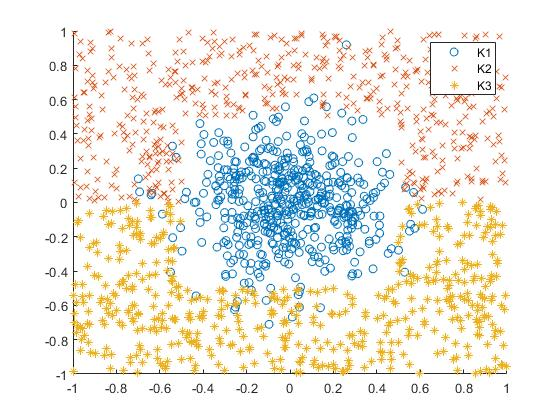
\includegraphics[width=6cm]{Resources/klasaRazvrstavanje}
                \captionof{figure}{Razvrstavanje po klasama}

    \end{center}
    
    Pošto imamo tri različite klase koje mogu biti prediktovane, \inlinecode{One-Hot Encoding} se nameće kao dobra ideja. OHE nam pomaže da lakše izvlačimo i upoređujemo podatke prilikom treniranja, a kasnije i korišćenja mreže. 
        \end{solution}

    \begin{solution}{}
        \subsection*{Razdvajanje dataseta na trening i test skupove}
    Sledeće što radimo jeste razbijanje skupa podataka koji nam je dat na 2 manja, nesrazmerna skupa. Veći skup će biti trening skup, a manji test skup. Test skup postoji da bismo mogli da procenimo performanse naše mreže na do sada neviđenim podacima. Mreža može biti previše "naviknuta" na trening podatke i performanse u realnim uslovima mogu da budu mnogo lošije od performansi prilikom treninga.
    
     \begin{center}
        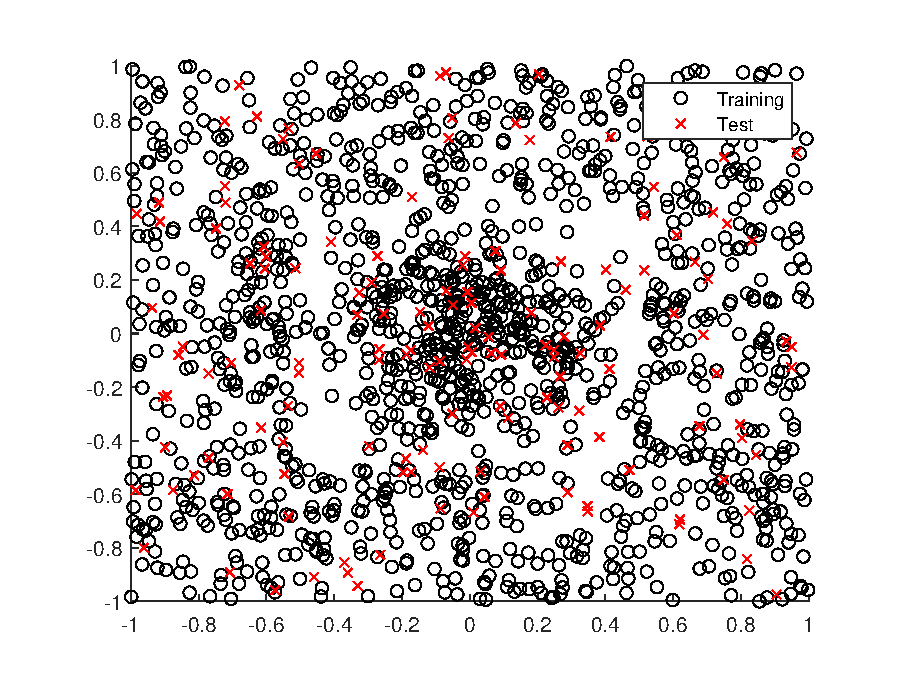
\includegraphics[width=14cm]{Resources/trainingvstest}
                \captionof{figure}{Trening i test skup}

    \end{center}
    Za ovaj projekat je korišćen odnos $90 ; 10$, odnosno 90\% podataka je bilo korišćeno za trening, a 10\% za procenu performansi neuralne mreže. Kod razdvajanja na trening i test skup jako je bitno da su podaci nasumično odabrani. Ako odbirci nisu dobro izmešani, može se desiti da recimo trening skup bude sačinjen samo od podataka koji pripadaju istoj klasi, pa samim tim test jednostavno nije merodavan.
    \end{solution}
    \newpage
    \begin{solution}{}
    \subsection*{Komparacija različitih arhitektura neuralnih mreža}
    Pre nego što kreiramo same mreže, bitno je odabrati i fiksirati hiperparametre koji će biti korišćeni u \underline{svakoj} mreži. Za ovaj projekat, parametri su:
    \begin{itemize}
        \item Broj epoha = $800$
        \item Maksimalna dozvoljena greška = $10^{-4}$
        \item Minimalni dozvoljeni gradijent = $10^{-6}$
    \end{itemize}
    Zadate su tri arhitekture:
    \begin{itemize}
        \item $[4,3,3]$ - Korektno optimizovana arhitektura
        \item $[1,2,1]$ - Primer arhitekture koja dovodi do \inlinecode{underfitting}-a
        \item $[9, 12, 16]$ - Primer arhitekture koja dovodi do \inlinecode{overfitting}-a
    \end{itemize}
    \subsubsection*{Underfitting}
    Neuralna mreža nam previše generalizuje. Ne možemo da se oslonimo na nju da predviđa korektno. U našem slučaju, mreža je imala 3 sloja oblika 1, 2, 1. To jednostavno nije dovoljan broj neurona da sa sigurnošću predviđa na osnovu zadatih parametera.
    Dalje možemo videti \inlinecode{confusion matrix} trening i test skupova za ovu mrežu.
     \begin{center}
        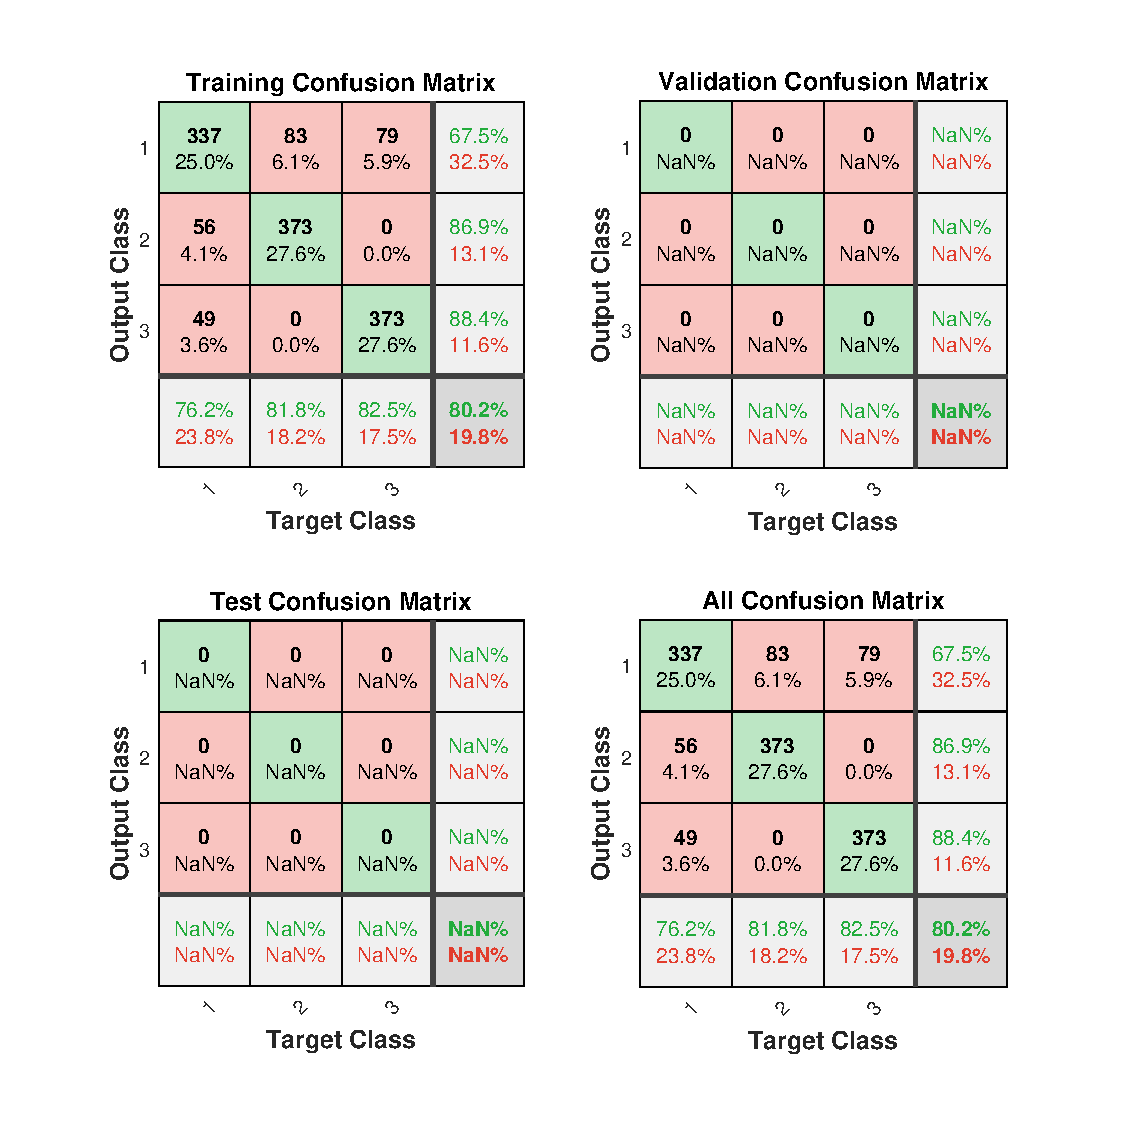
\includegraphics[width=12cm]{Resources/arch2cmtraining.eps}
                \captionof{figure}{Confusion matrix \inlinecode{underfitting} treninga}
    \end{center}
    \begin{center}
        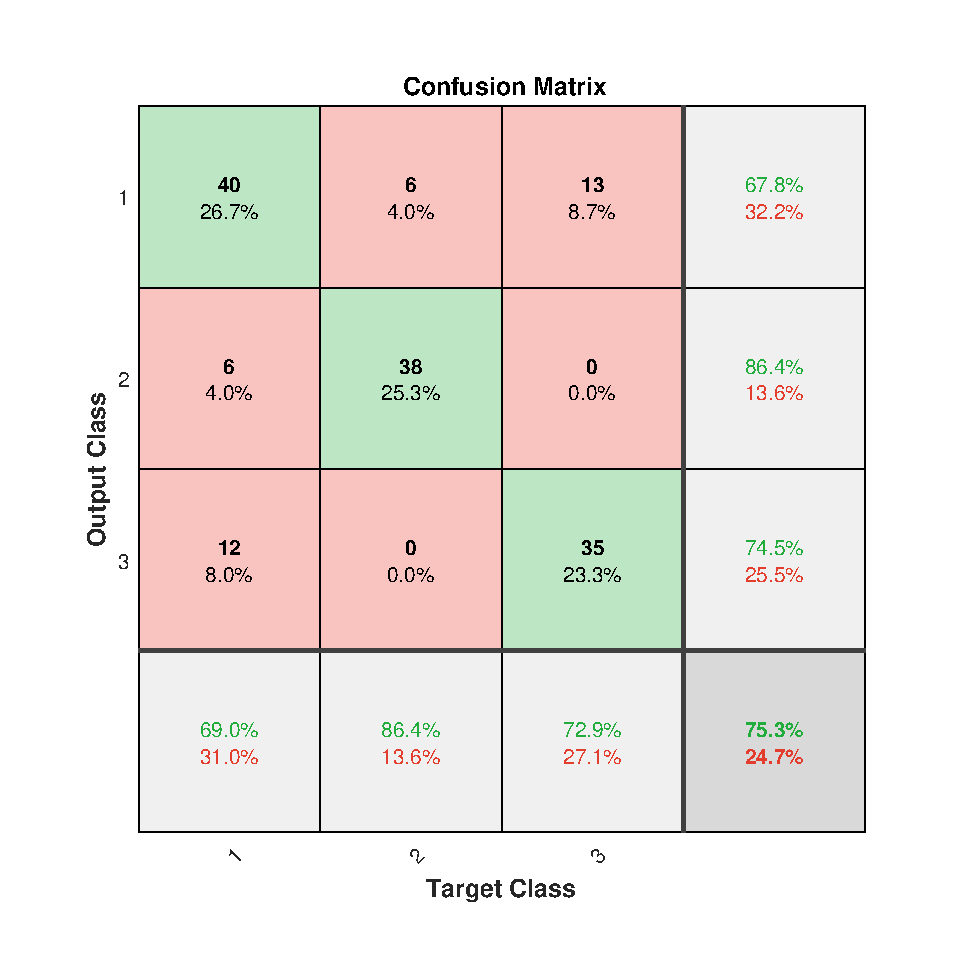
\includegraphics[width=12cm]{Resources/arch2cmtest.eps}
                \captionof{figure}{Confusion matrix \inlinecode{underfitting} testa}
    \end{center}
    Kao što vidimo, na test skupu je naša mreža imala 75.3\%, što je izuzetno loš rezultat. Čak je i na trening setu imala loše rezultat sa 80.2\%. Ostaje samo da se vidi granica odlučivanja.
        \begin{center}
        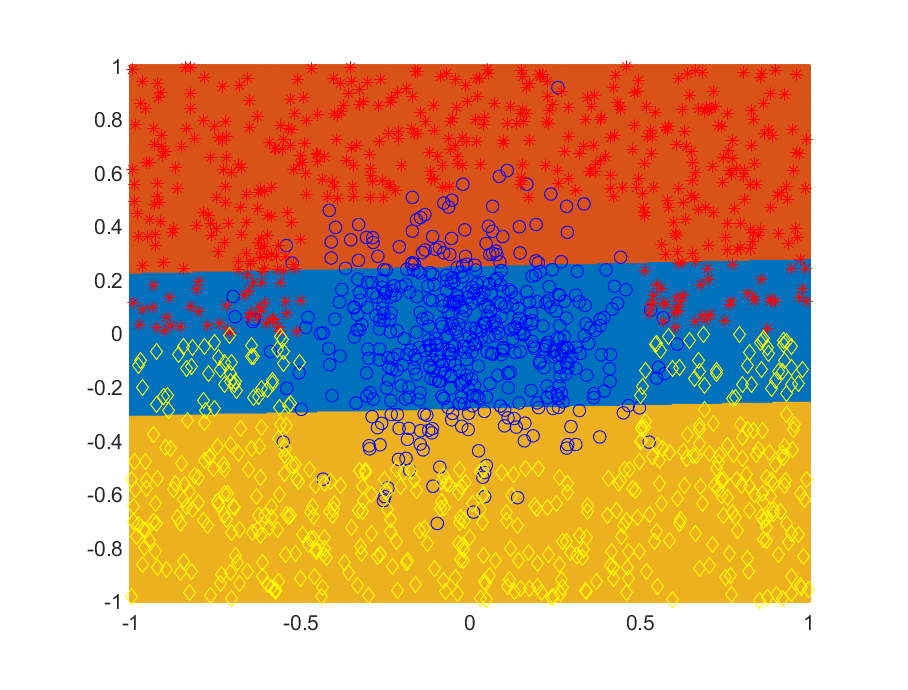
\includegraphics[width=7.5cm]{Resources/arch2limits.eps}
                \captionof{figure}{Granica odlučivanja za \inlinecode{underfitting} arhitekturu}
    \end{center}
    Po granicama odlučivanja jasnso vidimo da je mreža daleko od upotrebljive.
    \subsubsection*{Overfitting}
    Neuralna mreža je previše specijalizovana. Naučila je trening skup "previše dobro". Za određene klase traži vrlo specfične vrednosti. Nema previše odstupanja od trening seta.
    Dalje možemo videti \inlinecode{confusion matrix} trening i test skupova za ovu mrežu.
     \begin{center}
        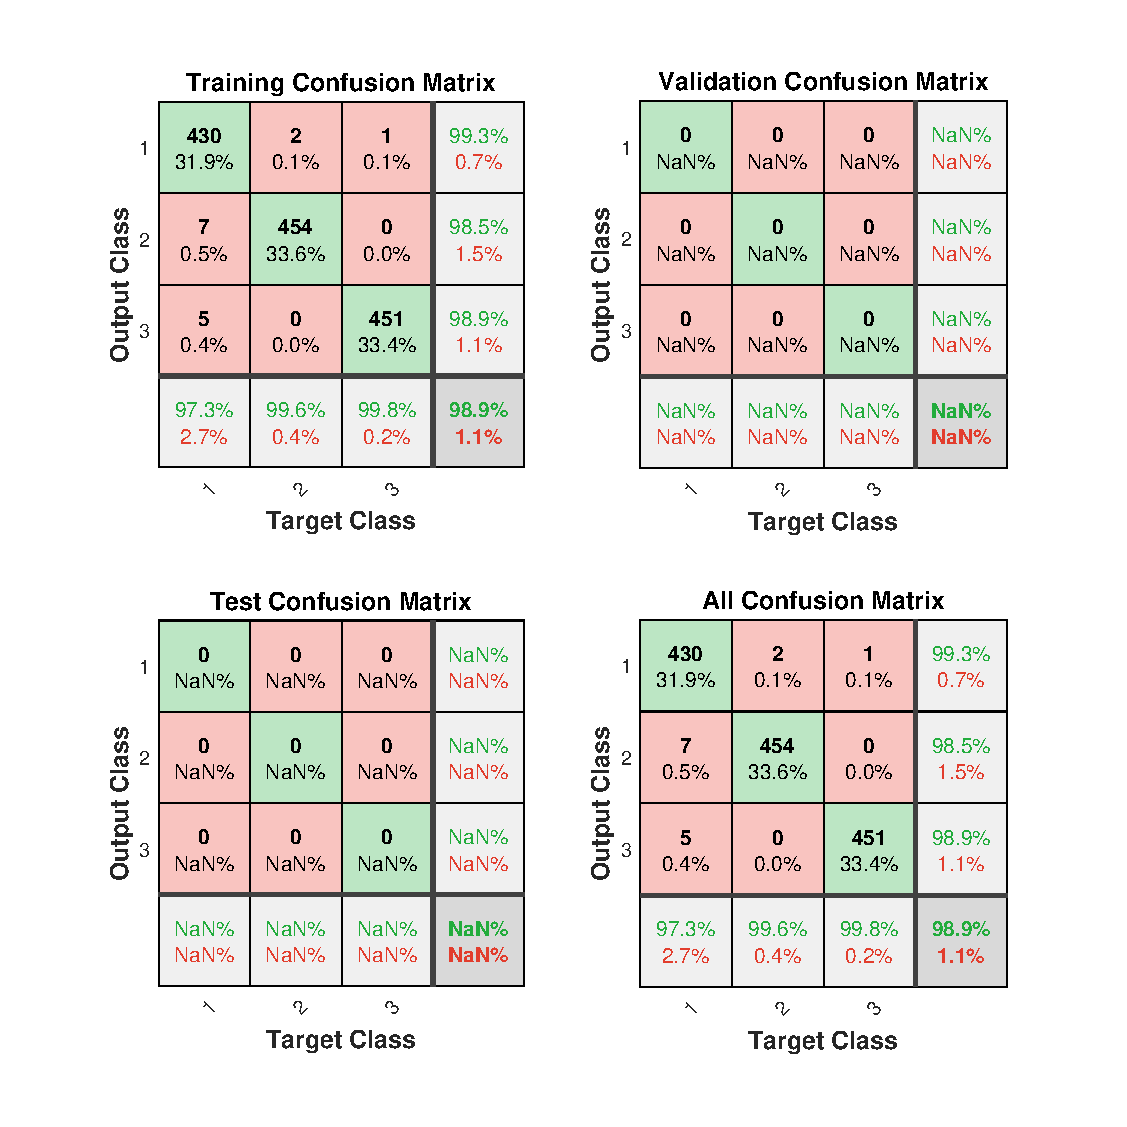
\includegraphics[width=16cm]{Resources/arch3cmtraining.eps}
                \captionof{figure}{Confusion matrix \inlinecode{overfitting} treninga}
    \end{center}
    \vspace{8cm}
    \begin{center}
        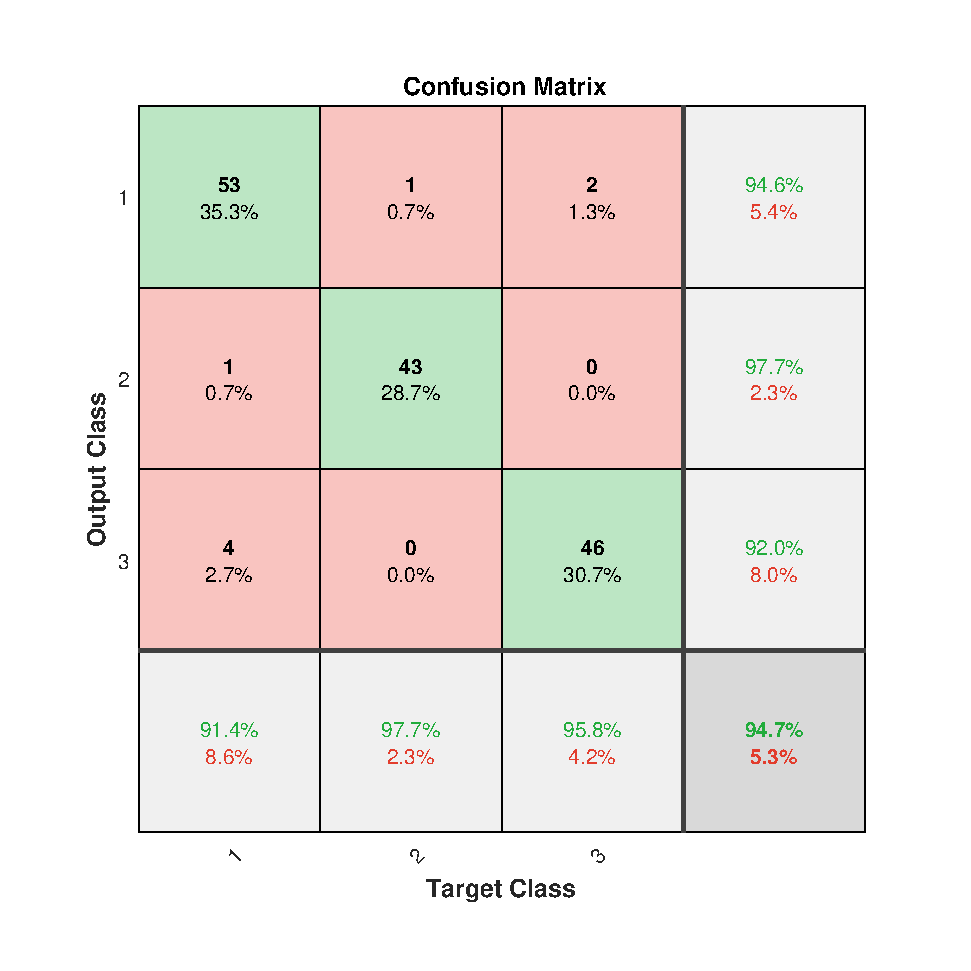
\includegraphics[width=12cm]{Resources/arch3cmtest.eps}
                \captionof{figure}{Confusion matrix \inlinecode{overfitting} testa}
    \end{center}
    Trening ima tačnost od 98.9\%, dok test set daje tačnost od 94.7\% što, posle brojeva iz \inlinecode{underfitting} dela, ne izgleda strašno ali odstupanje od 4.2\% je i dalje poprilično veliko i nezanemarljivo.
        \begin{center}
        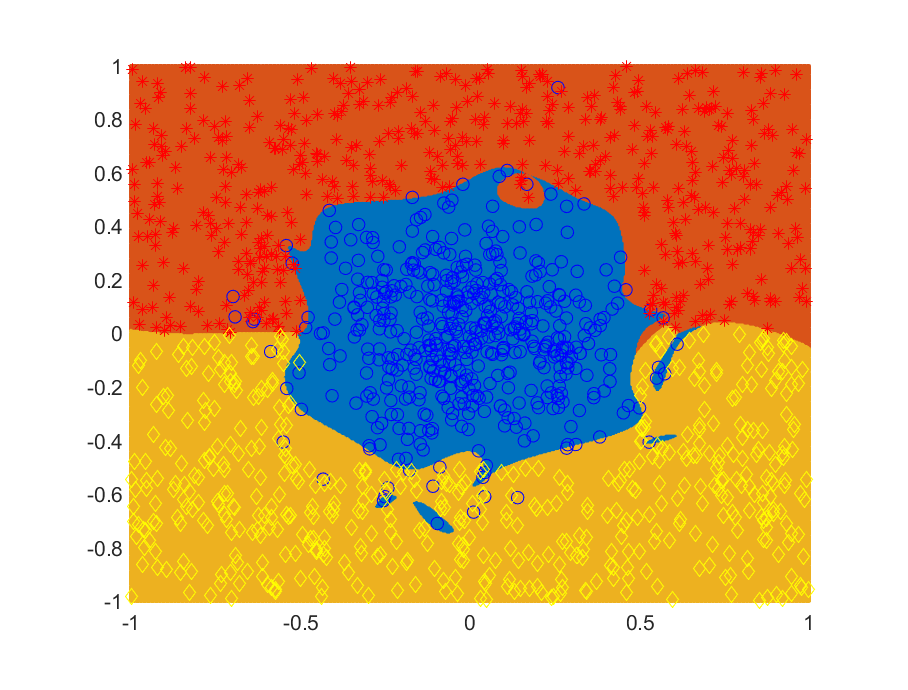
\includegraphics[width=10cm]{Resources/arch3limits.eps}
                \captionof{figure}{Granica odlučivanja za \inlinecode{underfitting} arhitekturu}
    \end{center}
    \subsubsection*{Korektno isplanirana arhitektura}
    Neuralna mreža je ne generalizuje previše, ali nije ni tako specifična u svojim zahtevima. U veoma velikom broju slučajeva može da predvidi klasu na osnovu zadatih parametara
    Dalje možemo videti \inlinecode{confusion matrix} trening i test skupova za ovu mrežu.
     \begin{center}
        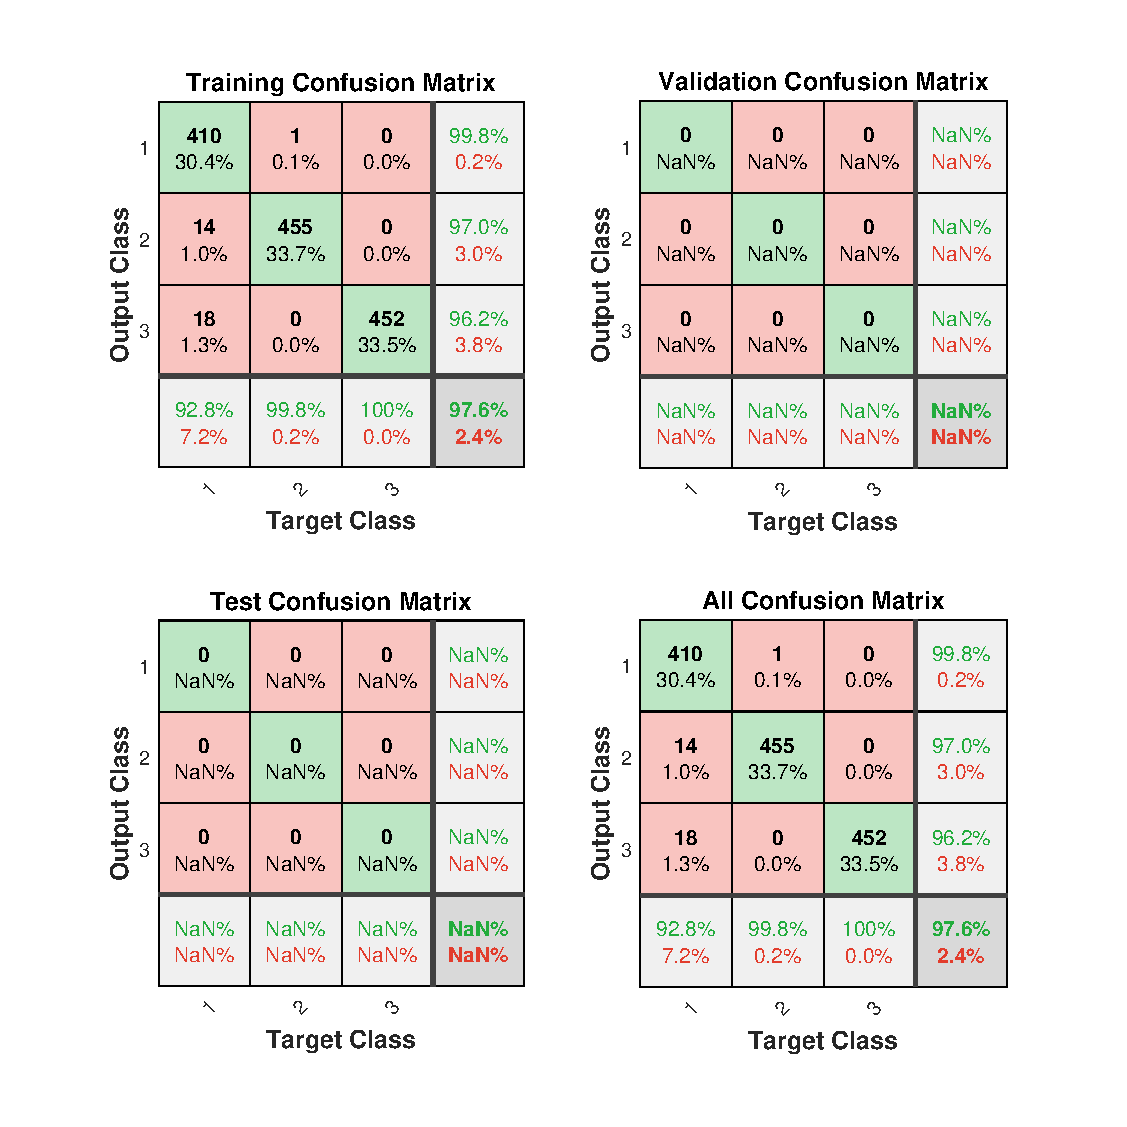
\includegraphics[width=16cm]{Resources/arch1cmtraining.eps}
                \captionof{figure}{Confusion matrix \inlinecode{overfitting} treninga}
    \end{center}
    \vspace{7cm}
    \begin{center}
        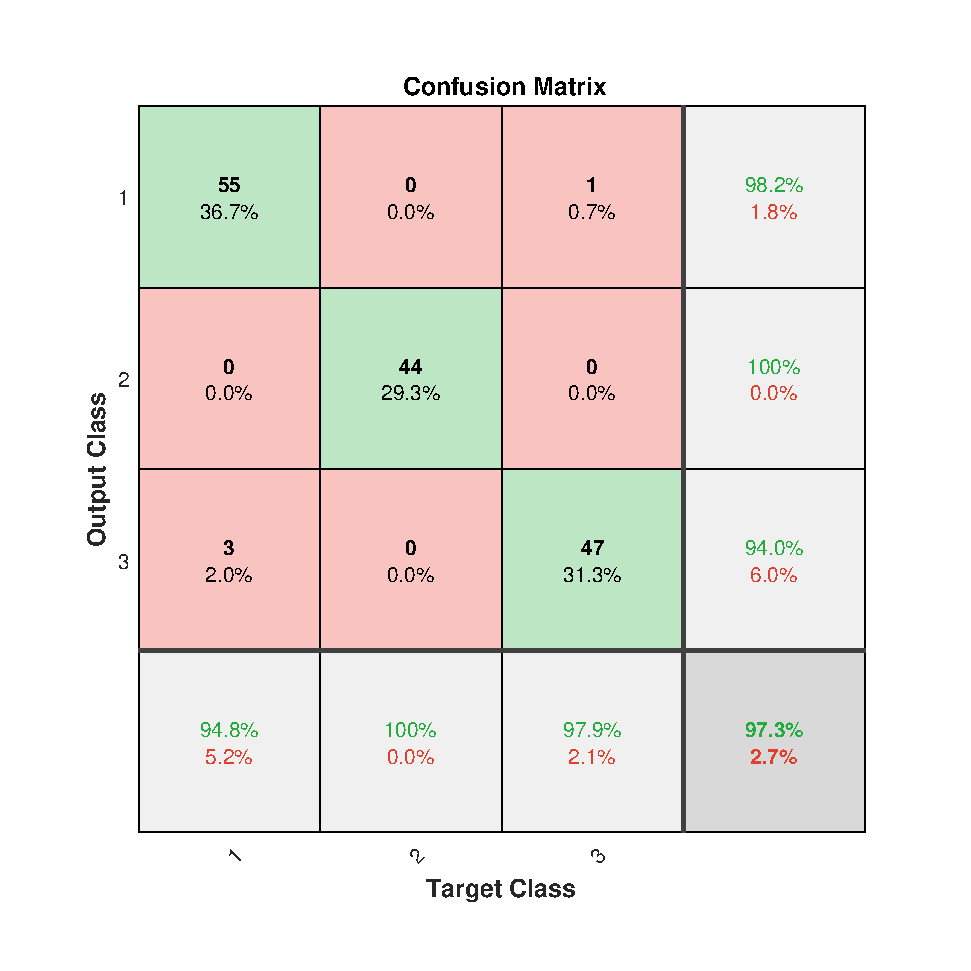
\includegraphics[width=12cm]{Resources/arch1cmtest.eps}
                \captionof{figure}{Confusion matrix \inlinecode{overfitting} testa}
    \end{center}
    Trening ima tačnost od 97.6\%, što je manje nego u slučaju \inlinecode{overfittinga}-a, ali test set daje tačnost od 97.3\%. \textit{Performance hit} je samo 0.3\%, što je prihvatljivo
        \begin{center}
        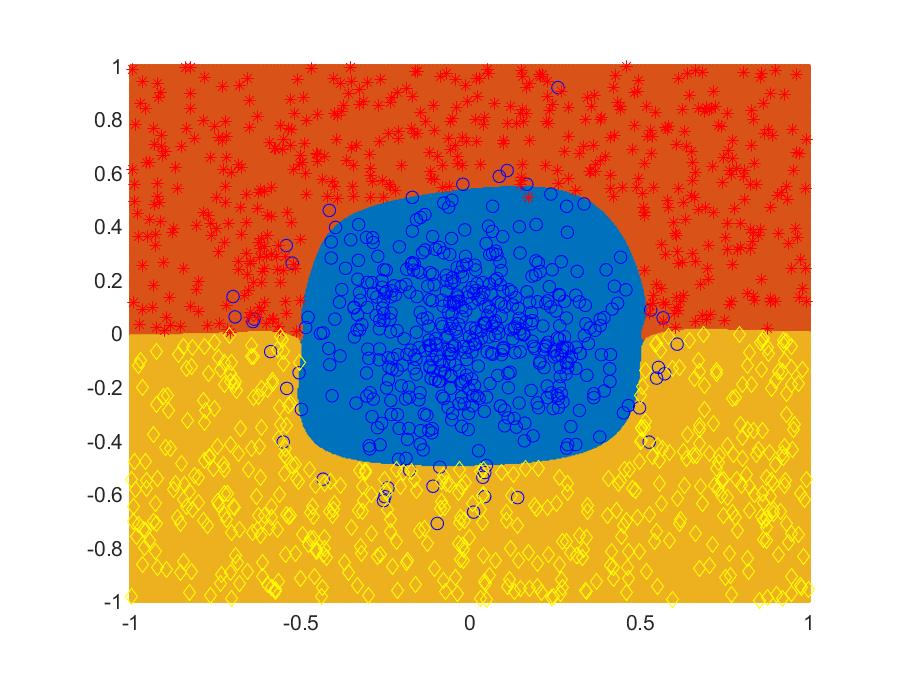
\includegraphics[width=10cm]{Resources/arch1limits.eps}
                \captionof{figure}{Granica odlučivanja }
    \end{center}
    \end{solution}

    
    \begin{eComment}{}
    Uporedili smo performanse tri vrlo različite arhitekture neuralnih mreža i potvrdili naša očekivanja. Idealna neuralna mreža balansira između generalizacija i specifikacija jako dobro, ne ideći nikada ni u jedan od ekstrema. \inlinecode{underfitted} mreža je loša u svakom pogledu, ni trening ni test performanse joj nisu dobre, sa velikim padom performansi na test setu. \inlinecode{Overfitted} mreža je odlično radila na trening setu, ali je pad performansi na test setu bio prevelik da bismo je uzeli u obzir. Treća mreža je napravila balans između prve dve, nije imala bolje performanse od \inlinecode{overfitted} mreže na trening skupu, ali je pad performansi na test setu bio izrazito mali. Možemo reći da je treća mreža na optimalan način klasifikuje podatke.
    \end{eComment}
    \newpage
    \begin{problem}{2}
    Za ovaj projekat nam je zadat \inlinecode{dataset} iz realnog života. 
    Formula za \inlinecode{dataset} glasi:
    \begin{center}
        $(B_1 + B_2 + B_3 + B_4)  \quad mod \quad 5 + 1$,
    \end{center} gde je $B_1B_2B_3B_4$ broj indeksa. Za indeks 0331 se dobija \inlinecode{dataset} \textit{JobChanges}.\\
    Na osnovu 11 različitih parametara procenjujemo da li zaposleni ima želju da napuste svoj trenutni posao. Parametri uključuju pol, mesto života, stepen stručne spreme, koliko često su subjekti menjali posao ranije... Na osnovu ovih informacija nama je cilj da vidimo da li je kandidat voljan da napusti svoj posao da bi došao u našu firmu.\\
    Osim podataka, zadata nam je i metoda optimizacije, kao i hiperparametri koje moramo odrediti metodom \inlinecode{cross-validation}. Formula za računanje glasi:
    \begin{center}
        $(B_1 + B_2 + B_3 + B_4)  \quad mod \quad 3 + 1$,
    \end{center} gde je $B_1B_2B_3B_4$ broj indeksa. Za indeks 0331 se dobija optimizacija sa adaptivnim stepenom obučavanja. Hiperparametri koje moramo odrediti su 
    \begin{itemize}
        \item Arhitektura mreže
        \item Stepen obučavanja
        \item Koeficijent regularizacije
        \item Težine klasa
    \end{itemize}
        Seeding je fiksan, zadat unapred i iznosi 200. 

        \end{problem}

    \begin{solution}{}
    \subsection*{Poređenje klasa}
        Klase nisu balansirane, mnogo je veći broj ljudi koji ne želi da se prebacuje sa svog radnog mesta.
        \begin{center}
        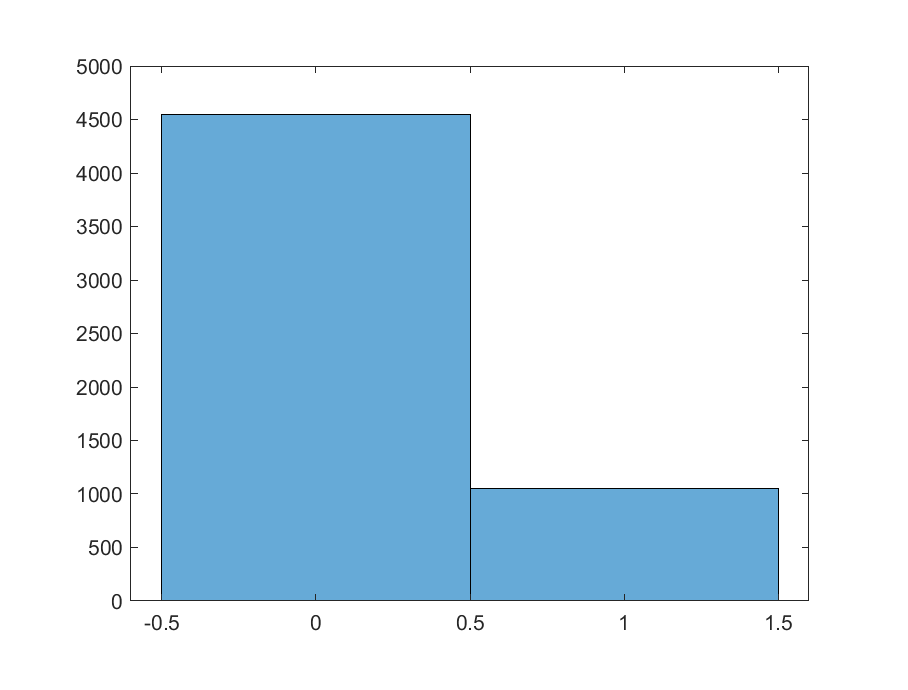
\includegraphics[width=8cm]{Resources/Dizbalans.eps}
                \captionof{figure}{Odnos klasa iz dataseta}
        \end{center}
        Jedna od opcija za rešavanje problema nebalansiranih klasa je dodavanje težina prilikom treniranja. Iako ima manje odbiraka klase 1, njihov uticaj je veći nego uticaj jednog odbirka klase 0. Ne znamo kolika je optimalna težina. Zadaćemo skup vrednosti i naći koja daje najbolje rezultate.
    
    
    \end{solution}
    \begin{solution}{}
    \subsection*{Početni parametri}
    Sledeći parametri su bili fiksni sve vreme:
    \begin{itemize}
        \item Broj epoha je iznosio 1000
        \item Ciljna greška je bila 0.0001
        \item Kriterijum za rano zaustavljanje je bio ako se 20 puta poveća greška na validacionom skupu
    \end{itemize}
    \textbf{NAPOMENA:} Iz nekog razloga MATLAB ne prikazuje validacioni skup na grafiku iako je sve na svom mestu. Zbog toga će na nekim graficima faliti informacije o validacionom skupu
    
    \end{solution}
    \begin{solution}{}
    \subsection*{Traženje optimalnih hiperparametara}
    Hiperparametri su uvek specifični za skup podataka, i ne postoji univerzalan broj koji se može koristiti. Jedino što nam preostaje je da probamo što više mogućnosti i vidimo koja je najbolja. Ovo naravno može potrajati jer treniranje neuralne mreže vrlo lako postane dugotrajan proces.
    Pošto nemamo previše vremena i želimo reproducibilne rezultate, prolazimo kroz malu količinu različitih hiperparametara. Ukupno ćemo imati 2250 treniranja neuralne mreže.
    Ovo su vrednosti koje smo prošli:
    \begin{itemize}
        \item Arhitekture: $[10, 5], [12, 6, 3], [4,6,4], [4,2,3], [4,4,4]$
        \item Težine: 1, 2, 5, 10
        \item Stepeni obučavanja: 0.01, 0.02, 0.03, 0.04, 0.05-0.55 sa inkrementom od 0.1
        \item Koeficijenti regularizacije: 0.1-1 sa inkrementom od 0.1
    \end{itemize}
    Nakon pretrage, najbolja kombinacija je bila:
    \begin{itemize}
        \item Arhitektura:$[4,4,4]$
        \item Težina: 1, 2, 5, 10\item Stepen obučavanja: 0.02
        \item Koeficijent regularizacije: 0.4
    \end{itemize}
    \end{solution}\newpage
    \begin{solution}{}
    \subsection*{Rezultati}
    \subsubsection*{Trening skup}
    Za gorenavedene parametre dobijamo sledeće performanse na trening skupu:
    \begin{itemize}
        \item \textbf{Preciznost/Accuracy} $= 85.1\%$
        \item \textbf{Osetljivost/Recall} $= 91.5\%$
        \item \textbf{F1} $= 0.90739$
    \end{itemize}
    \begin{center}
        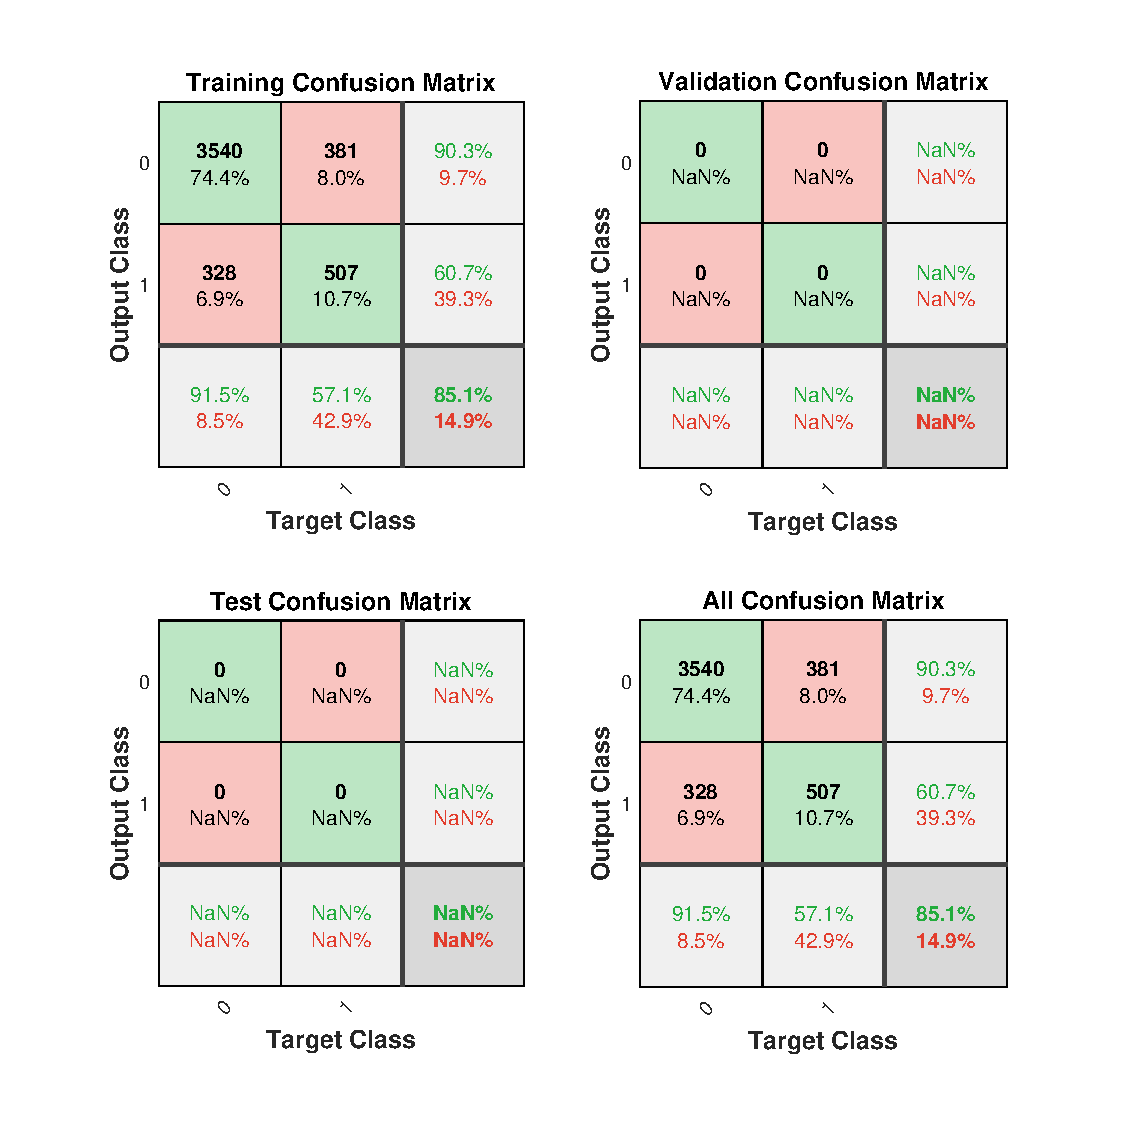
\includegraphics[width=15cm]{Resources/TrainingCM.eps}
                \captionof{figure}{\inlinecode{Confusion matrix} treninga}
    \end{center}
    \vspace{8cm}
    \newpage
        \subsubsection*{Test skup}

    Za test skup dobijamo:
    \begin{itemize}
        \item \textbf{Preciznost/Accuracy} $= 85.8\%$
        \item \textbf{Osetljivost/Recall} $= 92.2\%$
        \item \textbf{F1} $= 0.9065$
    \end{itemize}
    \begin{center}
        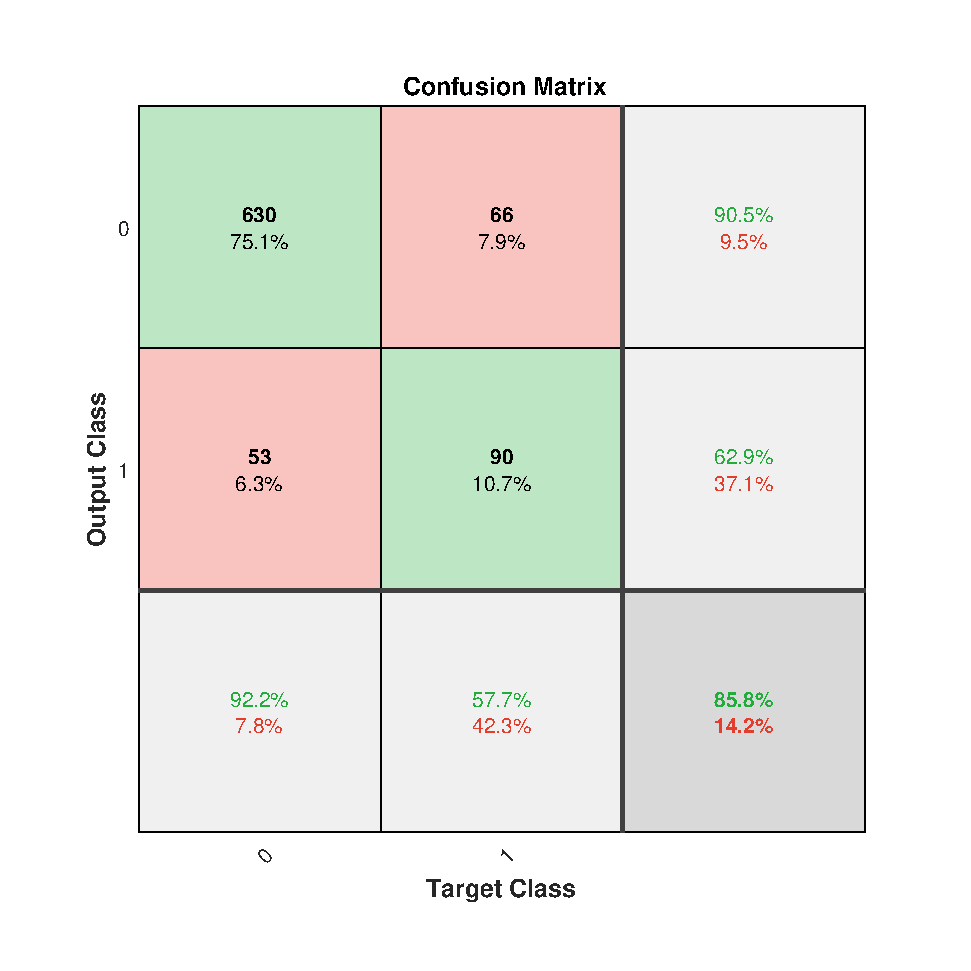
\includegraphics[width=7cm]{Resources/testCM.eps}
                \captionof{figure}{\inlinecode{Confusion matrix} testa}
    \end{center}
    Možemo zaključiti da je pad performansi mali i da je naša mreža konzistentna i na do sada neviđenim podacima. 
    \subsubsection*{Greška}
    Što se greške tiče, naš početni parametar je bio postavljen na 0.0001, ali je greška težila 0.1, što se može videti iz sledeće slike:
    \begin{center}
        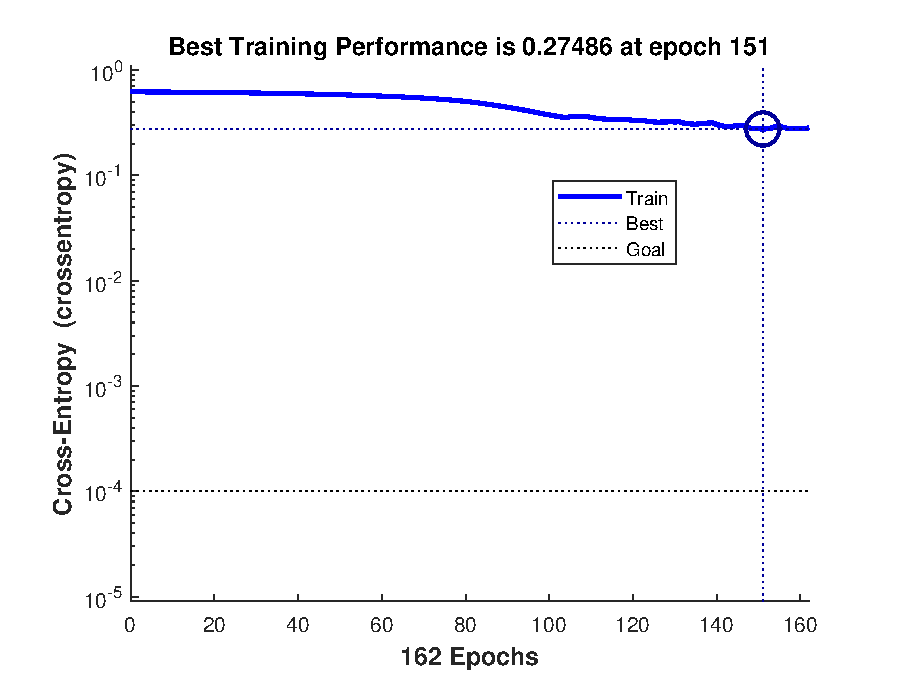
\includegraphics[width=7cm]{Resources/performance.eps}
                \captionof{figure}{Greška}
    \end{center}
    
    \end{solution}\newpage
    \begin{eComment}{}
    U ovom projektu smo tražili idealne vrednosti za hiperparametre, radeći na skupu podataka iz realnog života. Dobijeni rezultati su u velikoj meri očekivani, osim možda težina, za koje se ispostavilo da je najbolje ostaviti na 1. Sama tačnost naše neuralne mreže je poprilično dobra sa svojih $\sim$  85\%. Takođe, \inlinecode{performance hit} je bio negativan, performans je bio bolji na test setu.
    Sve u svemu, ova neuralna mreža može biti dobra strategija za neku veliku firmu, sa ogromnim brojem kandidata koji se intervjuišu i treniraju. Uz još veći \inlinecode{dataset} i, naravno, veću komputacionu moć, ova mreža se može značajno unaprediti.
    \end{eComment}
    

\end{document}